%**************************************************************************************
% License:
% CC BY-NC-SA 4.0 (http://creativecommons.org/licenses/by-nc-sa/4.0/)
%**************************************************************************************

\documentclass[notes]{beamer}

\mode<presentation> {

\usetheme{Madrid}

% Burnt orange
\definecolor{burntorange}{rgb}{0.8, 0.33, 0.0}
\colorlet{beamer@blendedblue}{burntorange}
% Pale yellow
\definecolor{paleyellow}{rgb}{1.0, 1.0, 0.953}
\setbeamercolor{background canvas}{bg=paleyellow}
% Secondary and tertiary palette
\setbeamercolor*{palette secondary}{use=structure,fg=white,bg=burntorange!80!black}
\setbeamercolor*{palette tertiary}{use=structure,fg=white,bg=burntorange!60!black}

% To remove the navigation symbols from the bottom of all slides uncomment this line
%\setbeamertemplate{navigation symbols}{}
}

\usepackage{amsmath}
\DeclareMathOperator*{\argmin}{arg\,min}
\DeclareMathOperator*{\argmax}{arg\,max}
\usepackage{bm}
\usepackage{booktabs} % Allows the use of \toprule, \midrule and \bottomrule in tables
\usepackage{breqn}
\usepackage{cleveref}
\usepackage{graphicx} % for figures
\usepackage[labelsep=space,tableposition=top]{caption}
\renewcommand{\figurename}{Fig.} 
\usepackage{caption,subcaption}% http://ctan.org/pkg/{caption,subcaption}
\usepackage{xcolor}
\usepackage{hyperref}

\AtBeginSection[]{
	\begin{frame}{Outline}
		\tableofcontents[
		currentsection,      % highlight the current section
		hideallsubsections   % show only section titles
		]
	\end{frame}
}

%----------------------------------------------------------------------------------------
%	TITLE PAGE
%----------------------------------------------------------------------------------------
\title[Physics-Informed Neural Networks]{Physics-Informed Neural Networks (PINNs)} 
\author{Krishna Kumar} % name
\institute[UT Austin] % institution 
{
University of Texas at Austin \\
\medskip
\textit{
  \url{krishnak@utexas.edu}} % Your email address
}
\date{} % Date, can be changed to a custom date

\begin{document}

\begin{frame}
\titlepage % title page as the first slide
\end{frame}

\begin{frame}
 \frametitle{Overview}
 \tableofcontents
\end{frame}

%----------------------------------------------------------------------------------------
% slides
%----------------------------------------------------------------------------------------

\section{The PINN Concept: Beyond Data-Only}

%------------------------------------------------
\begin{frame}
\frametitle{Learning Objectives}

\begin{itemize}
    \item Understand why standard neural networks fail for physics problems
    \item Learn how to incorporate physics into neural network training
    \item Master automatic differentiation for computing derivatives
    \item Compare data-driven vs physics-informed approaches
\end{itemize}

\vspace{1cm}
\centering
\href{https://colab.research.google.com/github/kks32-courses/ut-portugal-sciml/blob/main/docs/01-pinn/pinn.ipynb}{\beamergotobutton{Open Notebook: PINN}}

\end{frame}

%------------------------------------------------
\begin{frame}
\frametitle{The Problem: A Damped Harmonic Oscillator}

A mass $m$ on a spring (constant $k$) with damping (coefficient $c$). The displacement $u(t)$ satisfies:
\begin{equation*}
m \frac{d^2 u}{dt^2} + c \frac{du}{dt} + ku = 0
\end{equation*}
with initial conditions: $u(0) = 1$, $\frac{du}{dt}(0) = 0$.

\begin{figure}[ht]
	\centering
	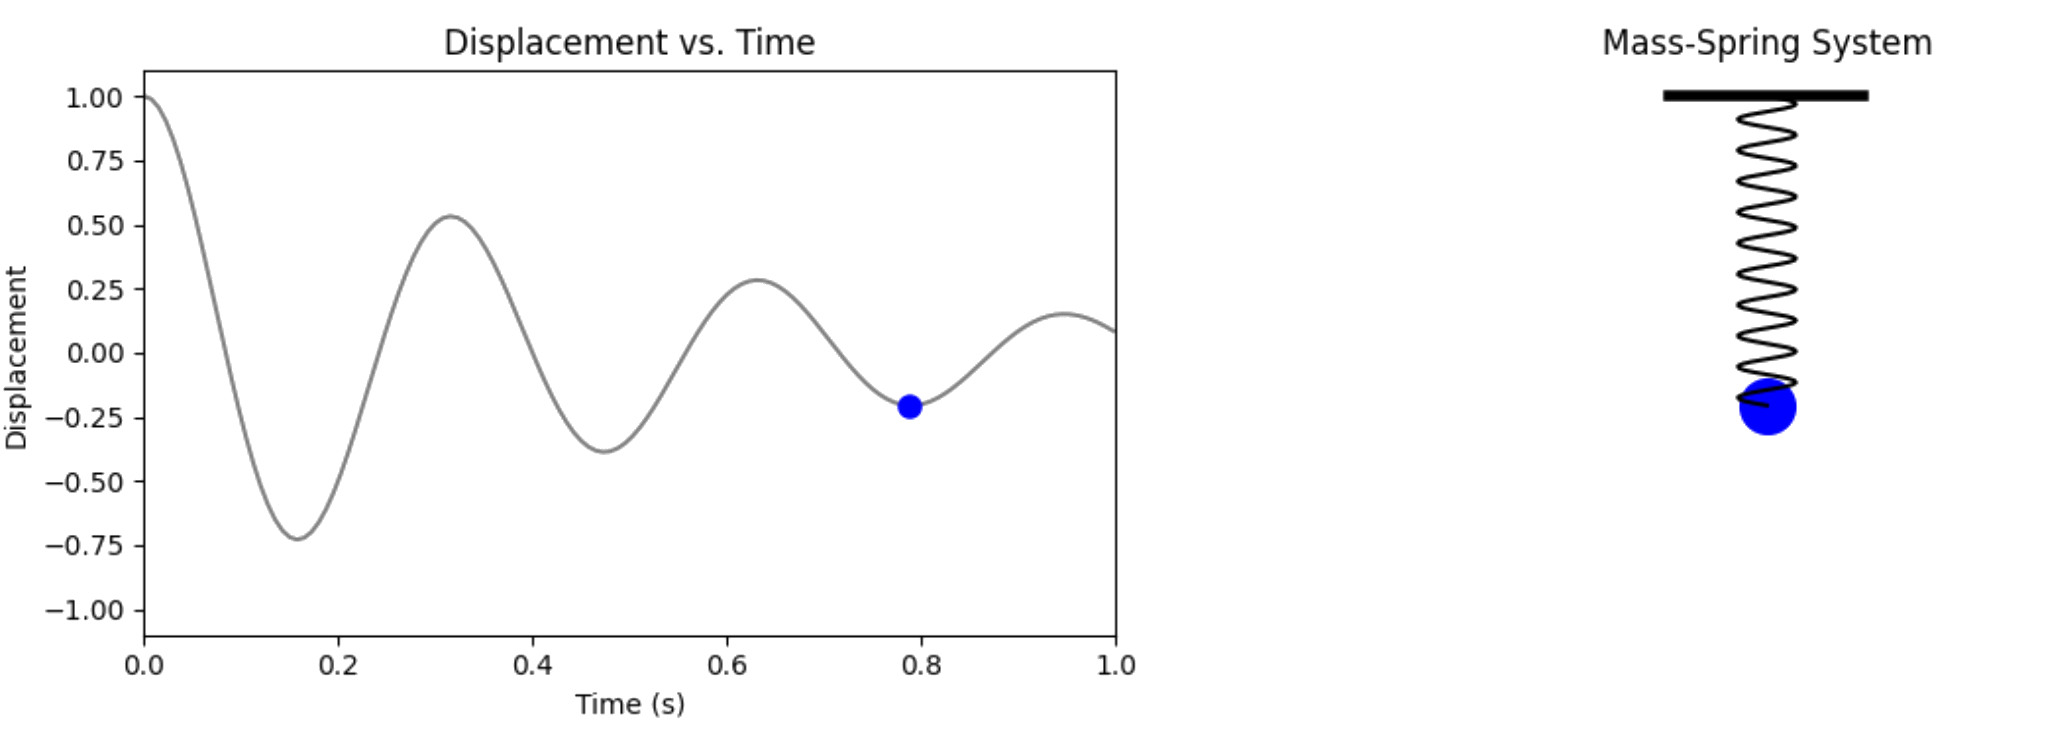
\includegraphics[width=0.5\textwidth]{figs/harmonic-oscillator.png}
	\caption*{A classic physics problem to illustrate PINNs.}
\end{figure}

\textbf{The Challenge:} Reconstruct the full solution $u(t)$ from a few sparse, noisy data points.

\end{frame}

%------------------------------------------------
\begin{frame}
\frametitle{Stage 1: The Data-Only Approach}

\textbf{Idea:} Train a standard neural network to fit the sparse data.

\begin{columns}[T]
    \begin{column}{0.5\textwidth}
        \textbf{Loss Function:} Mean Squared Error
        \begin{equation*}
        \mathcal{L}_{\text{data}}(\theta) = \frac{1}{N} \sum_{i=1}^N |\hat{u}_\theta(t_i) - u_i|^2
        \end{equation*}
        
        \textbf{Architecture:}
        \begin{itemize}
            \item Input: Time $t$
            \item Hidden Layers: Tanh activations
            \item Output: Displacement $\hat{u}_\theta(t)$
        \end{itemize}
    \end{column}
    \begin{column}{0.5\textwidth}
        \begin{figure}[ht]
            \centering
            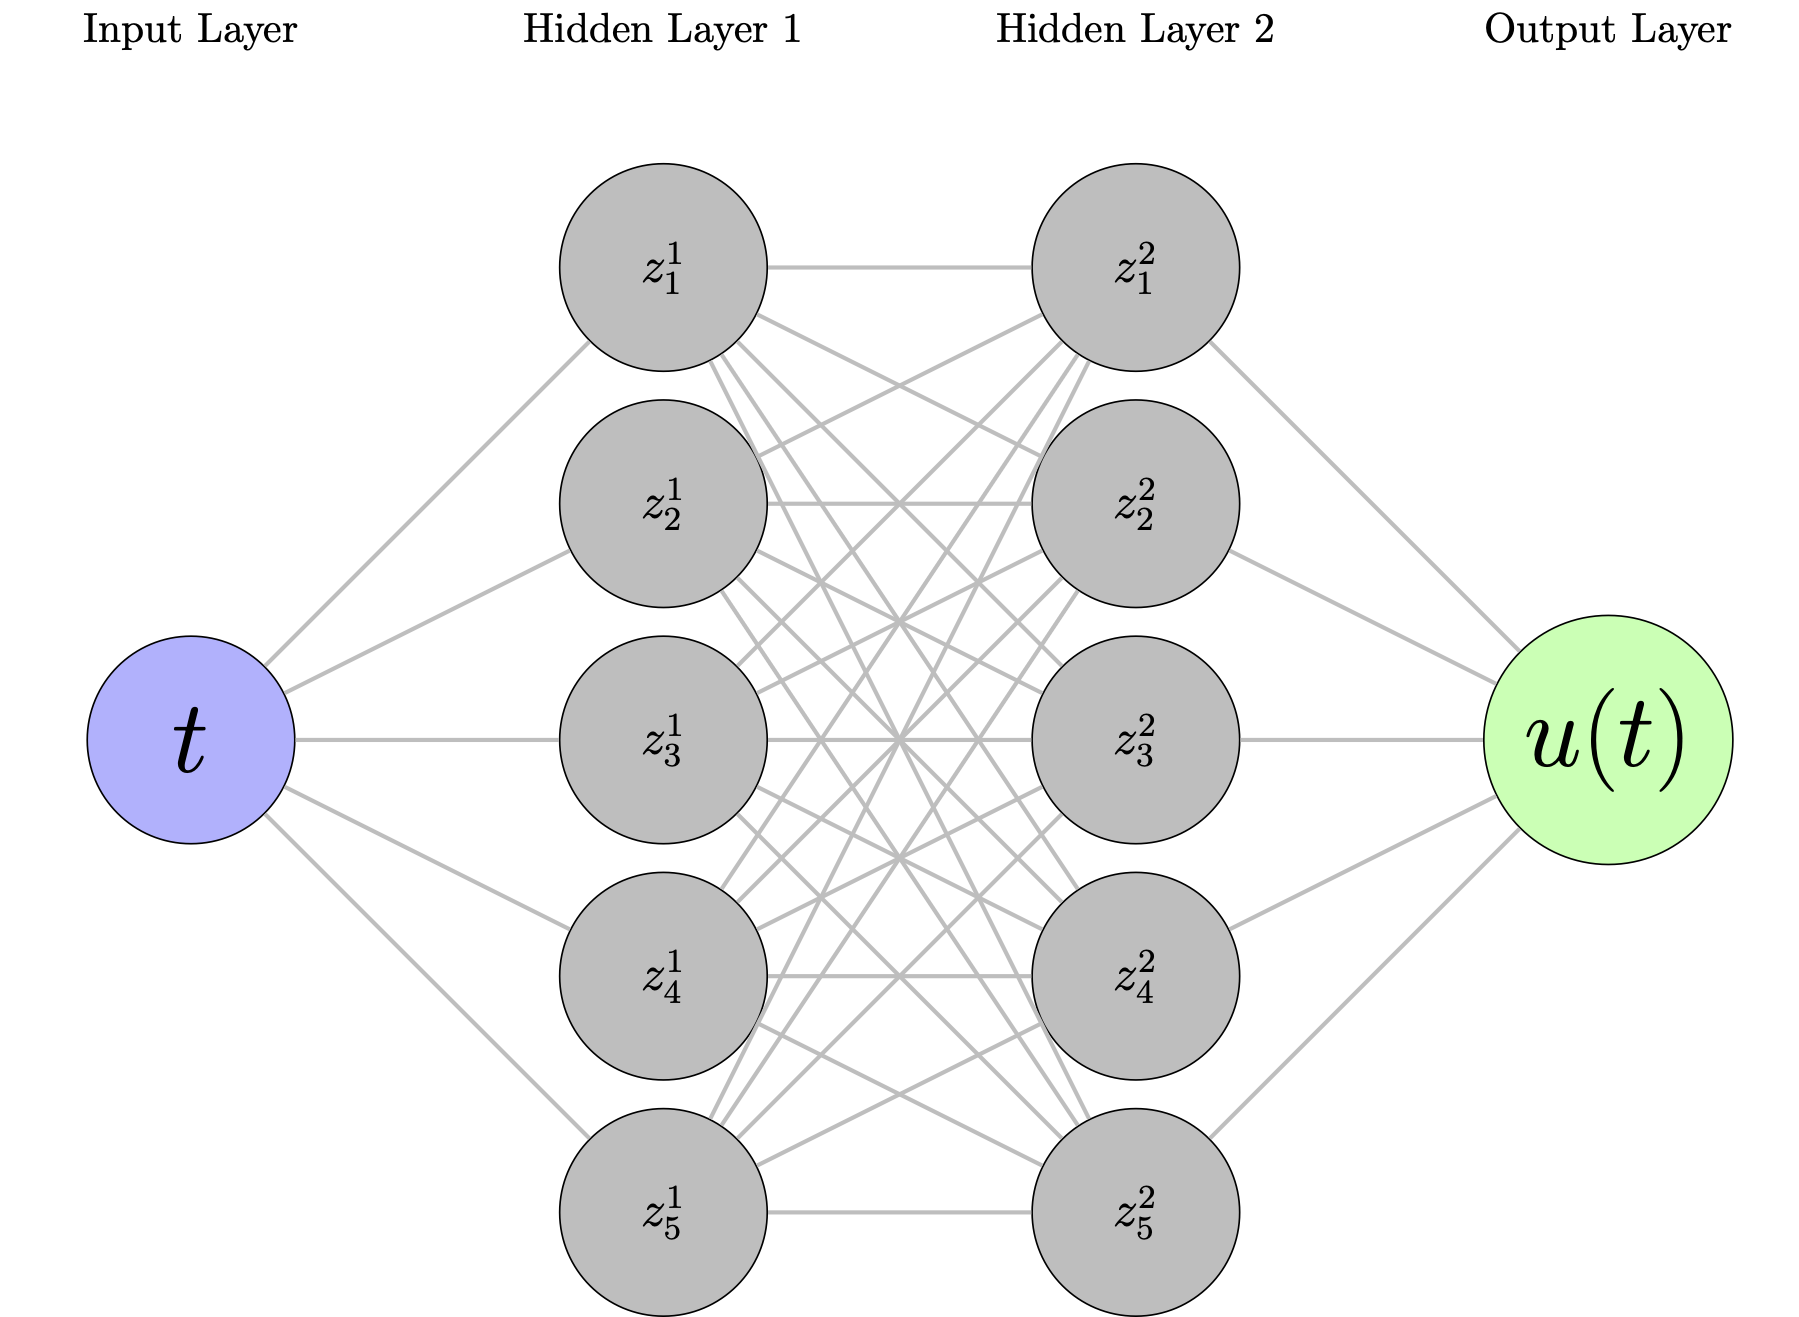
\includegraphics[width=\linewidth]{figs/oscillator-nn.png}
            \caption*{Standard NN for function fitting.}
        \end{figure}
    \end{column}
\end{columns}

\end{frame}

%------------------------------------------------
\begin{frame}
\frametitle{The Failure of the Data-Only Approach}

\textbf{Result:} The network fits the training points but fails catastrophically between them.

\begin{figure}[ht]
	\centering
	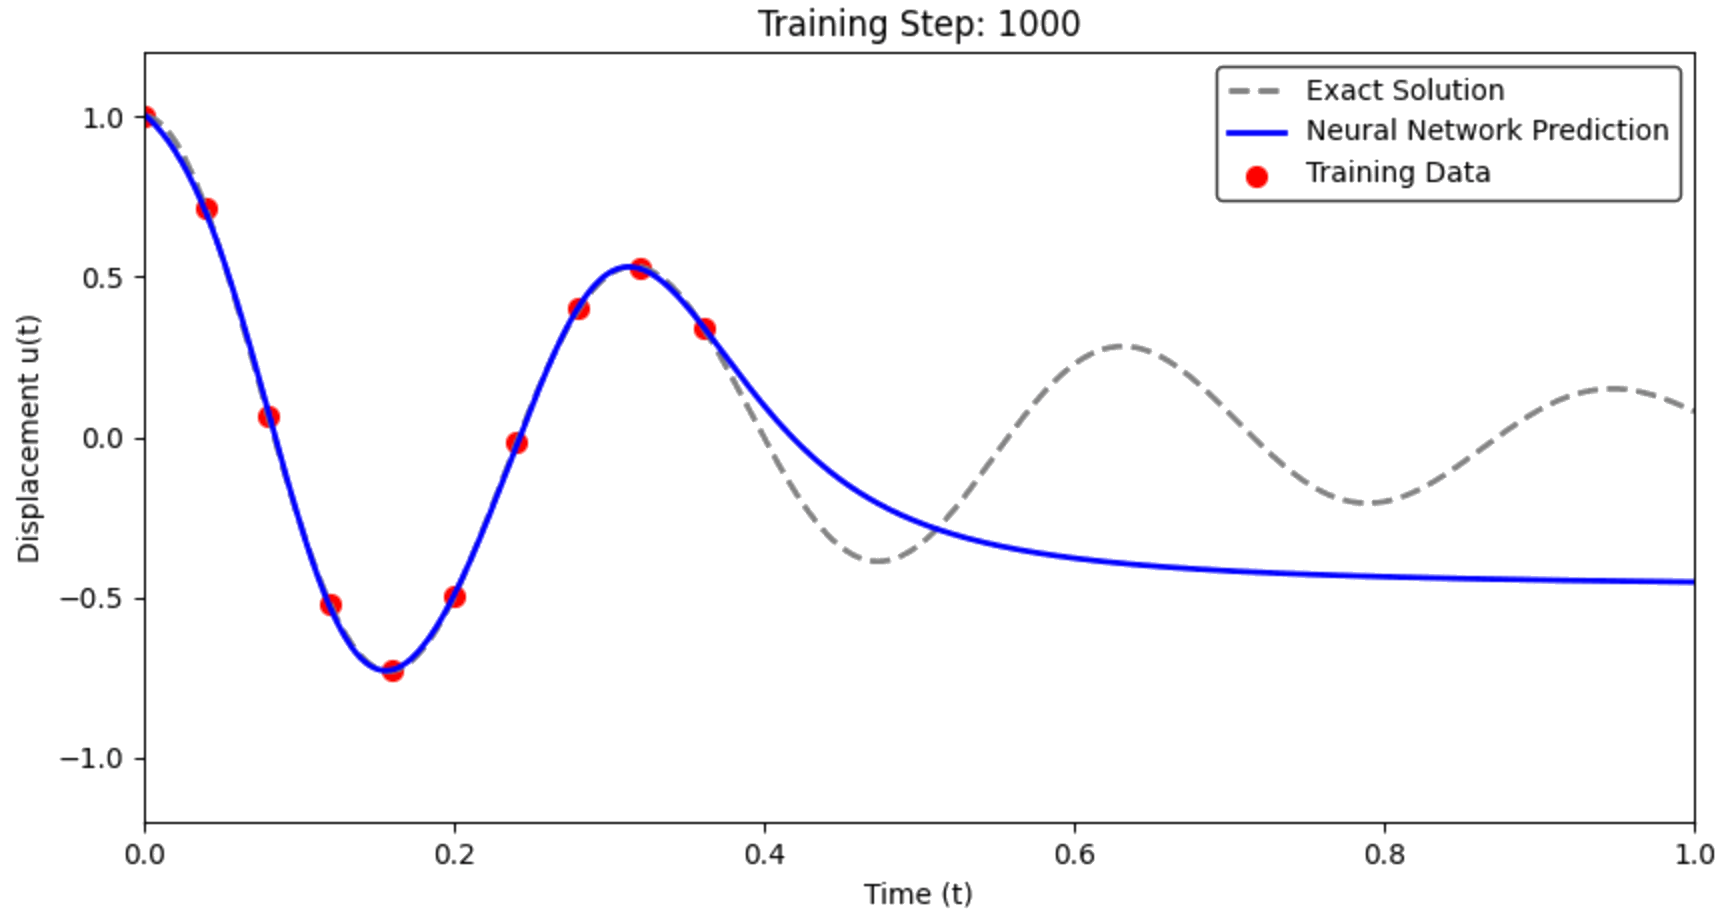
\includegraphics[width=0.9\textwidth]{figs/oscillator-result-nn.png}
	\caption*{The network overfits to the sparse data and does not respect the underlying physics.}
\end{figure}

\textbf{Conclusion:} The network has no knowledge of the governing laws of physics, leading to unphysical oscillations and poor generalization.

\end{frame}

%------------------------------------------------
\begin{frame}
\frametitle{Stage 2: Enter Physics-Informed Neural Networks}

\textbf{The Key Insight:} Don't just fit data. Enforce the differential equation itself!

\begin{columns}[T]
    \begin{column}{0.5\textwidth}
        \textbf{Physics Residual:}
        We define a residual based on the ODE:
        \begin{equation*}
        \mathcal{R}_\theta(t) = m\frac{d^2\hat{u}_\theta}{dt^2} + c\frac{d\hat{u}_\theta}{dt} + k\hat{u}_\theta
        \end{equation*}
        If the solution is correct, $\mathcal{R}_\theta(t)$ should be zero.
    \end{column}
    \begin{column}{0.5\textwidth}
        \begin{figure}[ht]
            \centering
            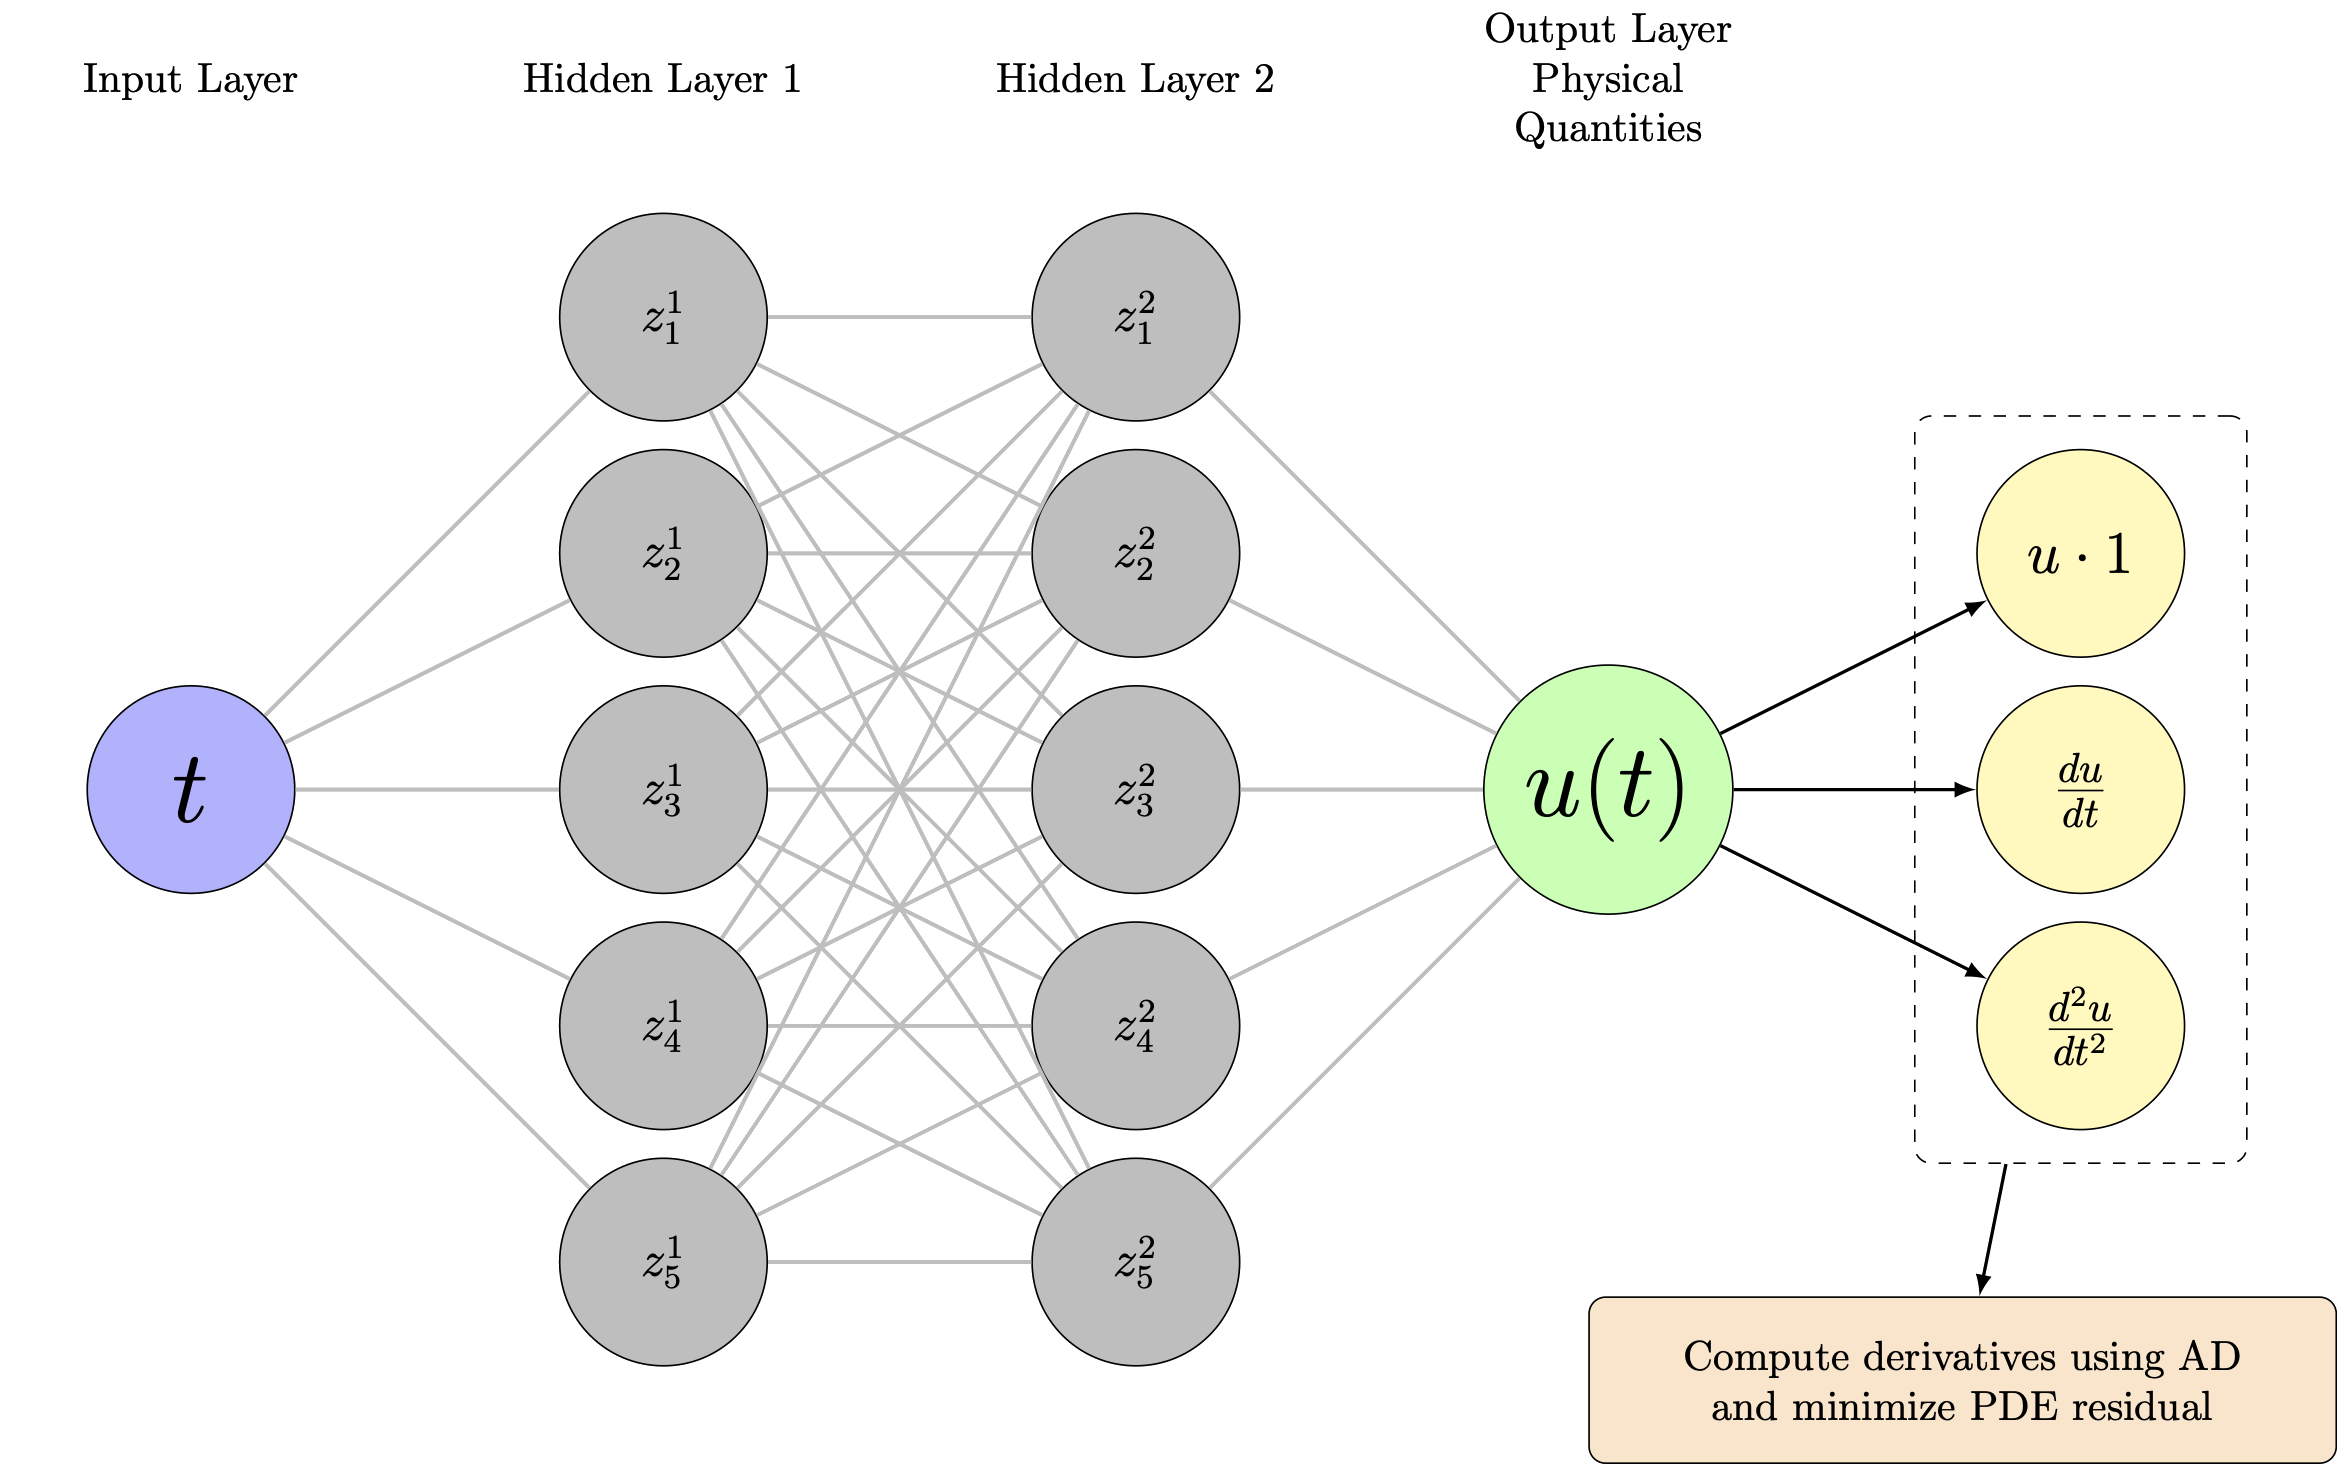
\includegraphics[width=\linewidth]{figs/oscillator-pinn-nn.png}
            \caption*{PINN architecture with physics loss.}
        \end{figure}
    \end{column}
\end{columns}

\end{frame}

%------------------------------------------------
\begin{frame}
\frametitle{The Complete PINN Loss Function}

The total loss is a combination of data fit and physics enforcement.

\textbf{Total Loss:}
\begin{equation*}
\mathcal{L}_{\text{total}}(\theta) = \mathcal{L}_{\text{data}}(\theta) + \lambda \mathcal{L}_{\text{physics}}(\theta)
\end{equation*}

\begin{block}{Data Loss}
Ensures the solution passes through the measurements.
\begin{equation*}
\mathcal{L}_{\text{data}}(\theta) = \frac{1}{N_{\text{data}}} \sum_{i=1}^{N_{\text{data}}} |\hat{u}_\theta(t_i) - u_i|^2
\end{equation*}
\end{block}

\begin{block}{Physics Loss}
Ensures the solution obeys the ODE at random "collocation" points.
\begin{equation*}
\mathcal{L}_{\text{physics}}(\theta) = \frac{1}{N_{\text{colloc}}} \sum_{j=1}^{N_{\text{colloc}}} |\mathcal{R}_\theta(t_j)|^2
\end{equation*}
\end{block}

The hyperparameter $\lambda$ balances the two terms.

\end{frame}

%------------------------------------------------
\begin{frame}
\frametitle{The Secret Weapon: Automatic Differentiation (AD)}

\textbf{Critical Question:} How do we compute $\frac{d\hat{u}_\theta}{dt}$ and $\frac{d^2\hat{u}_\theta}{dt^2}$?

\begin{alertblock}{Answer: Automatic Differentiation}
AD provides \textbf{exact} derivatives of the neural network output with respect to its input, by applying the chain rule through the computational graph.
\begin{itemize}
    \item No finite difference errors.
    \item Computationally efficient (especially reverse-mode AD).
    \item Built into modern frameworks (PyTorch, TensorFlow, JAX).
\end{itemize}
\end{alertblock}

\textbf{Example:} For $u(t) = \sin(t)$, AD can compute $u'(t)=\cos(t)$ and $u''(t)=-\sin(t)$ to machine precision.

\end{frame}

%------------------------------------------------
\begin{frame}
\frametitle{Theoretical Foundation: UAT for Sobolev Spaces}

\textbf{Classical UAT:} NNs can approximate any \textit{continuous function}.

\textbf{Problem:} For PDEs, we need to approximate functions \textbf{and their derivatives}.

\begin{block}{Extended Universal Approximation Theorem}
Neural networks with sufficiently smooth activation functions (e.g., $\tanh$, not ReLU) can approximate functions in \textbf{Sobolev spaces} $H^k(\Omega)$.
\begin{equation*}
\|u - \hat{u}_\theta\|_{H^k} < \epsilon
\end{equation*}
The Sobolev norm $\|u\|_{H^k}^2 = \sum_{|\alpha| \leq k} \|D^\alpha u\|_{L^2}^2$ measures the error in the function and all its derivatives up to order $k$.
\end{block}

\textbf{Why this matters:} For a $k^{th}$-order ODE/PDE, we need an activation function that is at least $k$ times differentiable ($C^k$). For our 2nd-order oscillator, we need a $C^2$ activation like $\tanh$.

\end{frame}

%------------------------------------------------
\begin{frame}
\frametitle{The Moment of Truth: Standard NN vs. PINN}

\begin{figure}[ht]
	\centering
	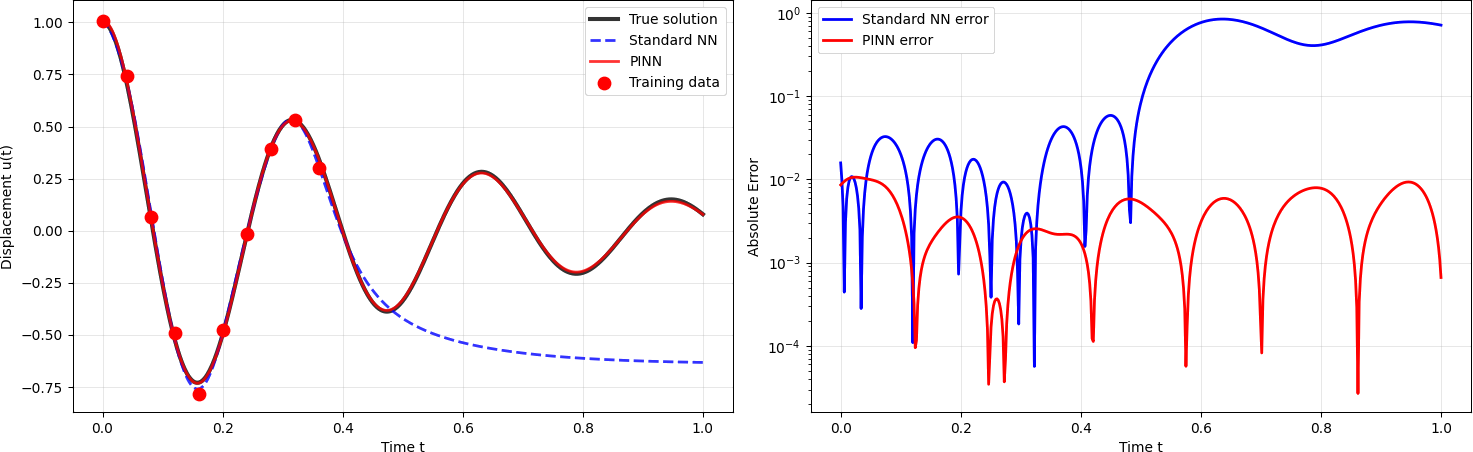
\includegraphics[width=\textwidth]{figs/pinn-nn-comparison.png}
	\caption*{Placeholder for the comparison plot from the notebook.}
\end{figure}

\textbf{Observation:}
\begin{itemize}
    \item \textbf{Standard NN:} Fits data points, but fails to generalize.
    \item \textbf{PINN:} Fits data points AND follows the physics, resulting in a globally accurate solution.
\end{itemize}

\end{frame}

%------------------------------------------------
\begin{frame}
\frametitle{Deep Dive: Derivative and Phase Portrait Analysis}

The ultimate test: Does the PINN learn physically consistent derivatives?

\begin{figure}[ht]
	\centering
	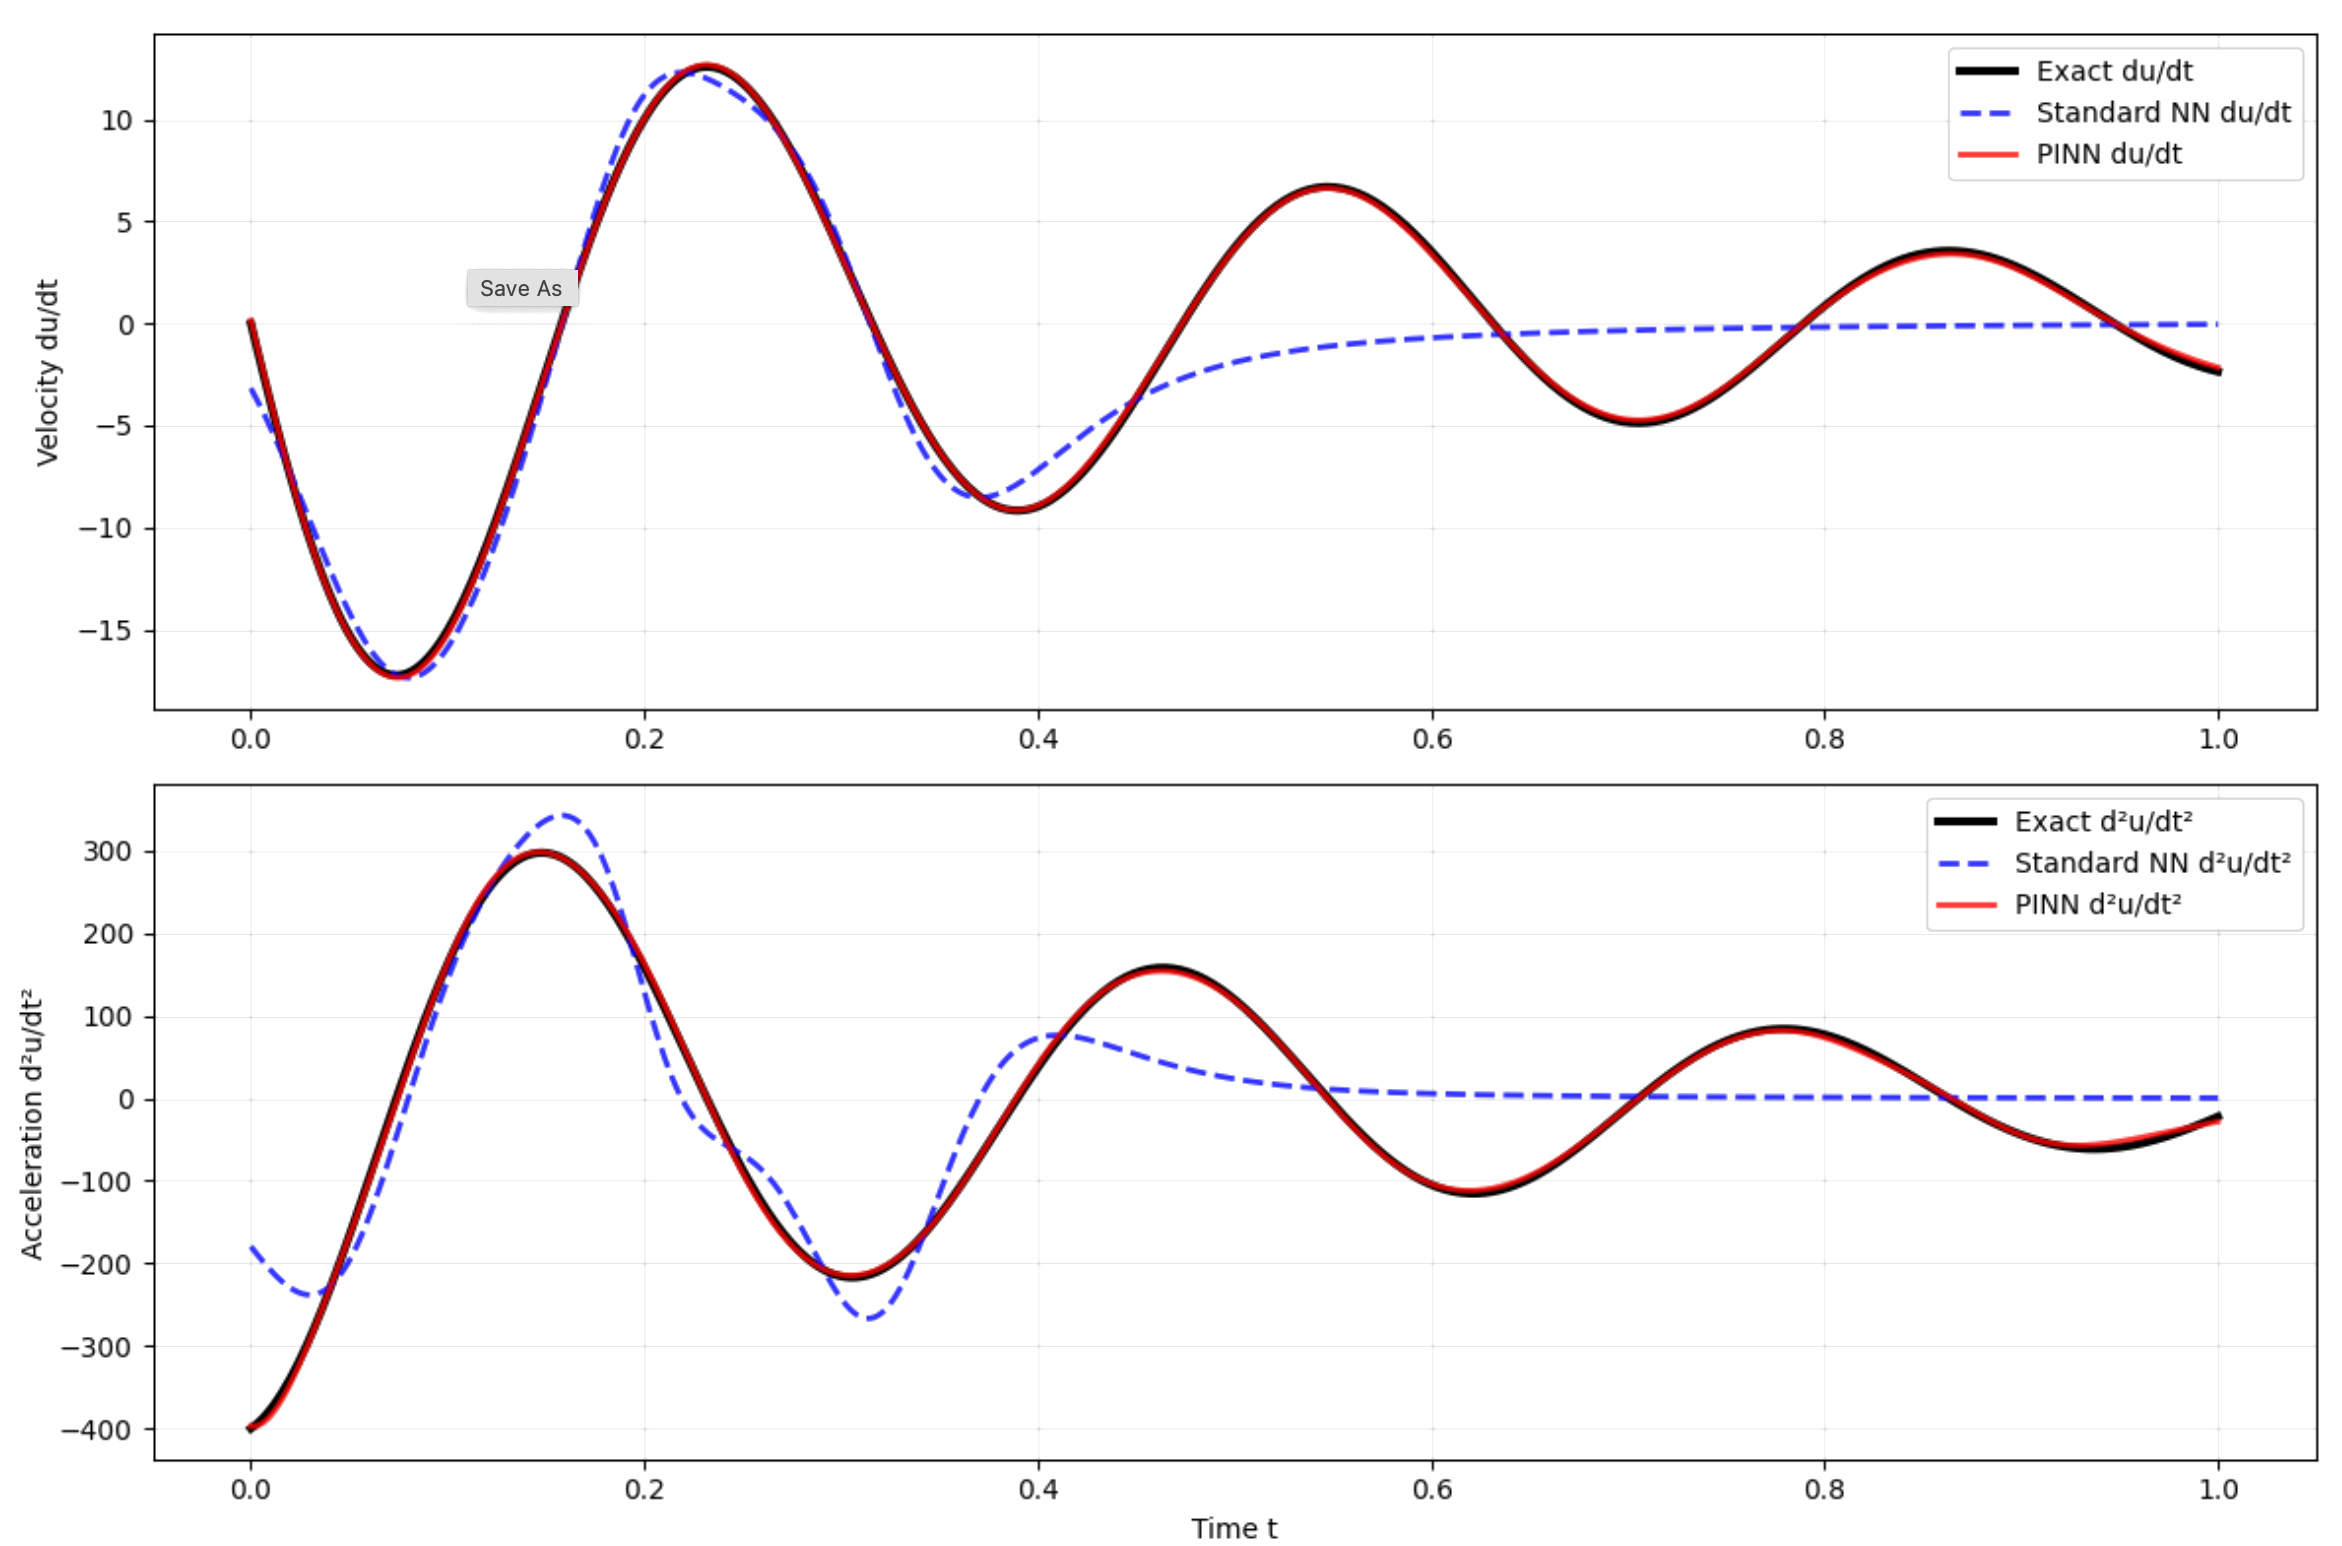
\includegraphics[width=\textwidth]{figs/derivative-comparison.png}
	\caption*{Derivative  plots.}
\end{figure}

\textbf{Result:} The PINN learns the correct velocity ($du/dt$) and acceleration ($d^2u/dt^2$).

\end{frame}

%------------------------------------------------
\begin{frame}
	\frametitle{Deep Dive: Derivative and Phase Portrait Analysis}
	
	The ultimate test: Does the PINN learn physically consistent derivatives?
	
	\begin{figure}[ht]
		\centering
		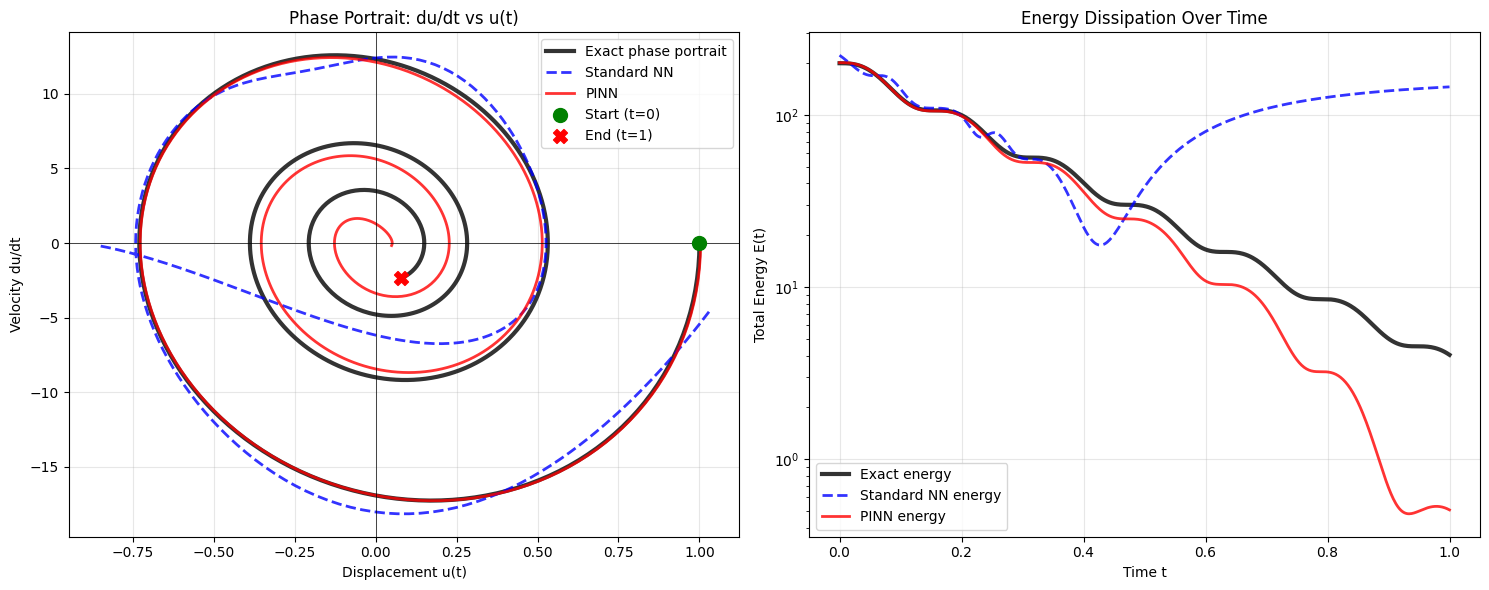
\includegraphics[width=\textwidth]{figs/oscillator-phase-portrait.png}
		\caption*{Phase portrait plots.}
	\end{figure}
	
	\textbf{Result:} The phase portrait (velocity vs. displacement) traces the correct physical trajectory (a spiral for a damped oscillator).
	
\end{frame}

%------------------------------------------------
\section{Enforcing Boundary Conditions}

%------------------------------------------------
\begin{frame}
\frametitle{The 1D Poisson Problem}

We now tackle a boundary value problem, the 1D Poisson equation:
\begin{equation*}
\frac{d^2u}{dx^2} + \pi \sin(\pi x) = 0, \quad \text{for } x \in [0, 1]
\end{equation*}
with Dirichlet boundary conditions (BCs):
\begin{equation*}
u(0) = 0 \quad \text{and} \quad u(1) = 0
\end{equation*}

\textbf{Goal:} Train a PINN to find the solution using only the governing equation and its BCs.

\vspace{1cm}
\centering
\href{https://colab.research.google.com/github/kks32-courses/ut-portugal-sciml/blob/main/docs/01-pinn/poisson.ipynb}{\beamergotobutton{Open Notebook: 1D Poisson}}

\end{frame}

%------------------------------------------------
\begin{frame}
\frametitle{Method 1: Soft Constraints}

Treat the boundary conditions as another component of the loss function.

\textbf{Total Loss:}
\begin{equation*}
\mathcal{L}_{\text{total}} = \mathcal{L}_{\text{PDE}} + \lambda_{BC} \mathcal{L}_{BC}
\end{equation*}

\begin{block}{Boundary Loss}
A mean squared error term that penalizes violations of the BCs.
\begin{equation*}
\mathcal{L}_{BC} = \frac{1}{N_{BC}} \sum_{i=1}^{N_{BC}} |\hat{u}_\theta(x_i) - u_{BC}|^2
\end{equation*}
\end{block}

\begin{alertblock}{Pros \& Cons}
\begin{itemize}
    \item[+]\textbf{Flexible:} Easy to implement for any type of BC (Dirichlet, Neumann, etc.).
    \item[-]\textbf{Approximate:} Satisfaction is not guaranteed, only encouraged.
    \item[-]\textbf{Tuning:} Requires careful tuning of the weight $\lambda_{BC}$.
\end{itemize}
\end{alertblock}

\end{frame}

%------------------------------------------------
\begin{frame}
\frametitle{Method 2: Hard Constraints}

Modify the network architecture to satisfy the BCs \textit{by construction}.

For our problem with $u(0)=0$ and $u(1)=0$, we can define a trial solution $\tilde{u}(x)$:
\begin{equation*}
\tilde{u}(x) = \underbrace{x(1-x)}_{D(x)} \cdot \underbrace{\text{NN}(x; \theta)}_{\text{Network Output}}
\end{equation*}
The distance function $D(x)$ is zero at the boundaries, forcing $\tilde{u}(x)$ to be zero there, regardless of the network's output.

\begin{alertblock}{Pros \& Cons}
\begin{itemize}
    \item[+]\textbf{Exact:} BCs are satisfied perfectly.
    \item[+]\textbf{Simpler Loss:} No need for $\mathcal{L}_{BC}$ or $\lambda_{BC}$, leading to more stable training.
    \item[-]\textbf{Inflexible:} Requires designing a specific trial function for the problem's geometry and BCs, which can be difficult for complex cases.
\end{itemize}
\end{alertblock}

\end{frame}

%------------------------------------------------
\begin{frame}
\frametitle{Comparison: Soft vs. Hard Constraints}

\begin{figure}[ht]
	\centering
	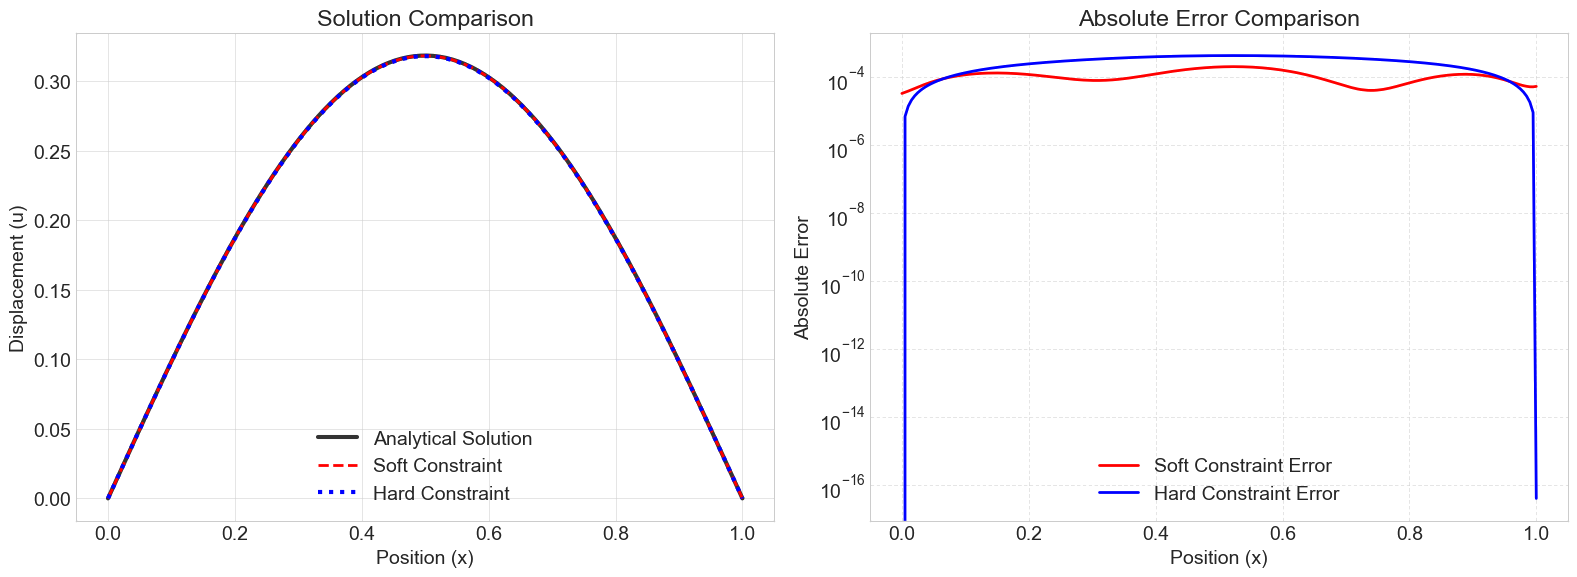
\includegraphics[width=\textwidth]{figs/poisson-soft-vs-hard.png}
	\caption*{Comparison plot of soft vs. hard constraint solutions and errors.}
\end{figure}

\textbf{Conclusion:}
\begin{itemize}
    \item Both methods achieve high accuracy.
    \item The hard constraint method shows slightly lower error and, by design, has zero error at the boundaries.
    \item For simple geometries and Dirichlet BCs, \textbf{hard constraints are often superior}.
    \item For complex problems, \textbf{soft constraints offer greater versatility}.
\end{itemize}

\end{frame}

%------------------------------------------------
\section{Inverse Problems: Discovering Physics}

%------------------------------------------------
\begin{frame}
\frametitle{Forward vs. Inverse Problems}

\begin{block}{Forward Problem}
\begin{itemize}
    \item \textbf{Given:} Full physical model (equations + parameters).
    \item \textbf{Find:} The solution $u(x,t)$.
    \item \textit{Example: Simulate temperature given thermal conductivity.}
\end{itemize}
\end{block}

\begin{block}{Inverse Problem}
\begin{itemize}
    \item \textbf{Given:} Sparse measurements of the solution $u(x,t)$.
    \item \textbf{Find:} Unknown physical parameters in the model.
    \item \textit{Example: Infer thermal conductivity from temperature measurements.}
\end{itemize}
\end{block}

\vspace{1em}
\centering
\href{https://colab.research.google.com/github/kks32-courses/ut-portugal-sciml/blob/main/docs/01-pinn/inverse-heat.ipynb}{\beamergotobutton{Open Notebook: Inverse Heat}}


\end{frame}

%------------------------------------------------
\begin{frame}
	\frametitle{Forward vs. Inverse Problems}
	
	\begin{figure}[ht]
		\centering
		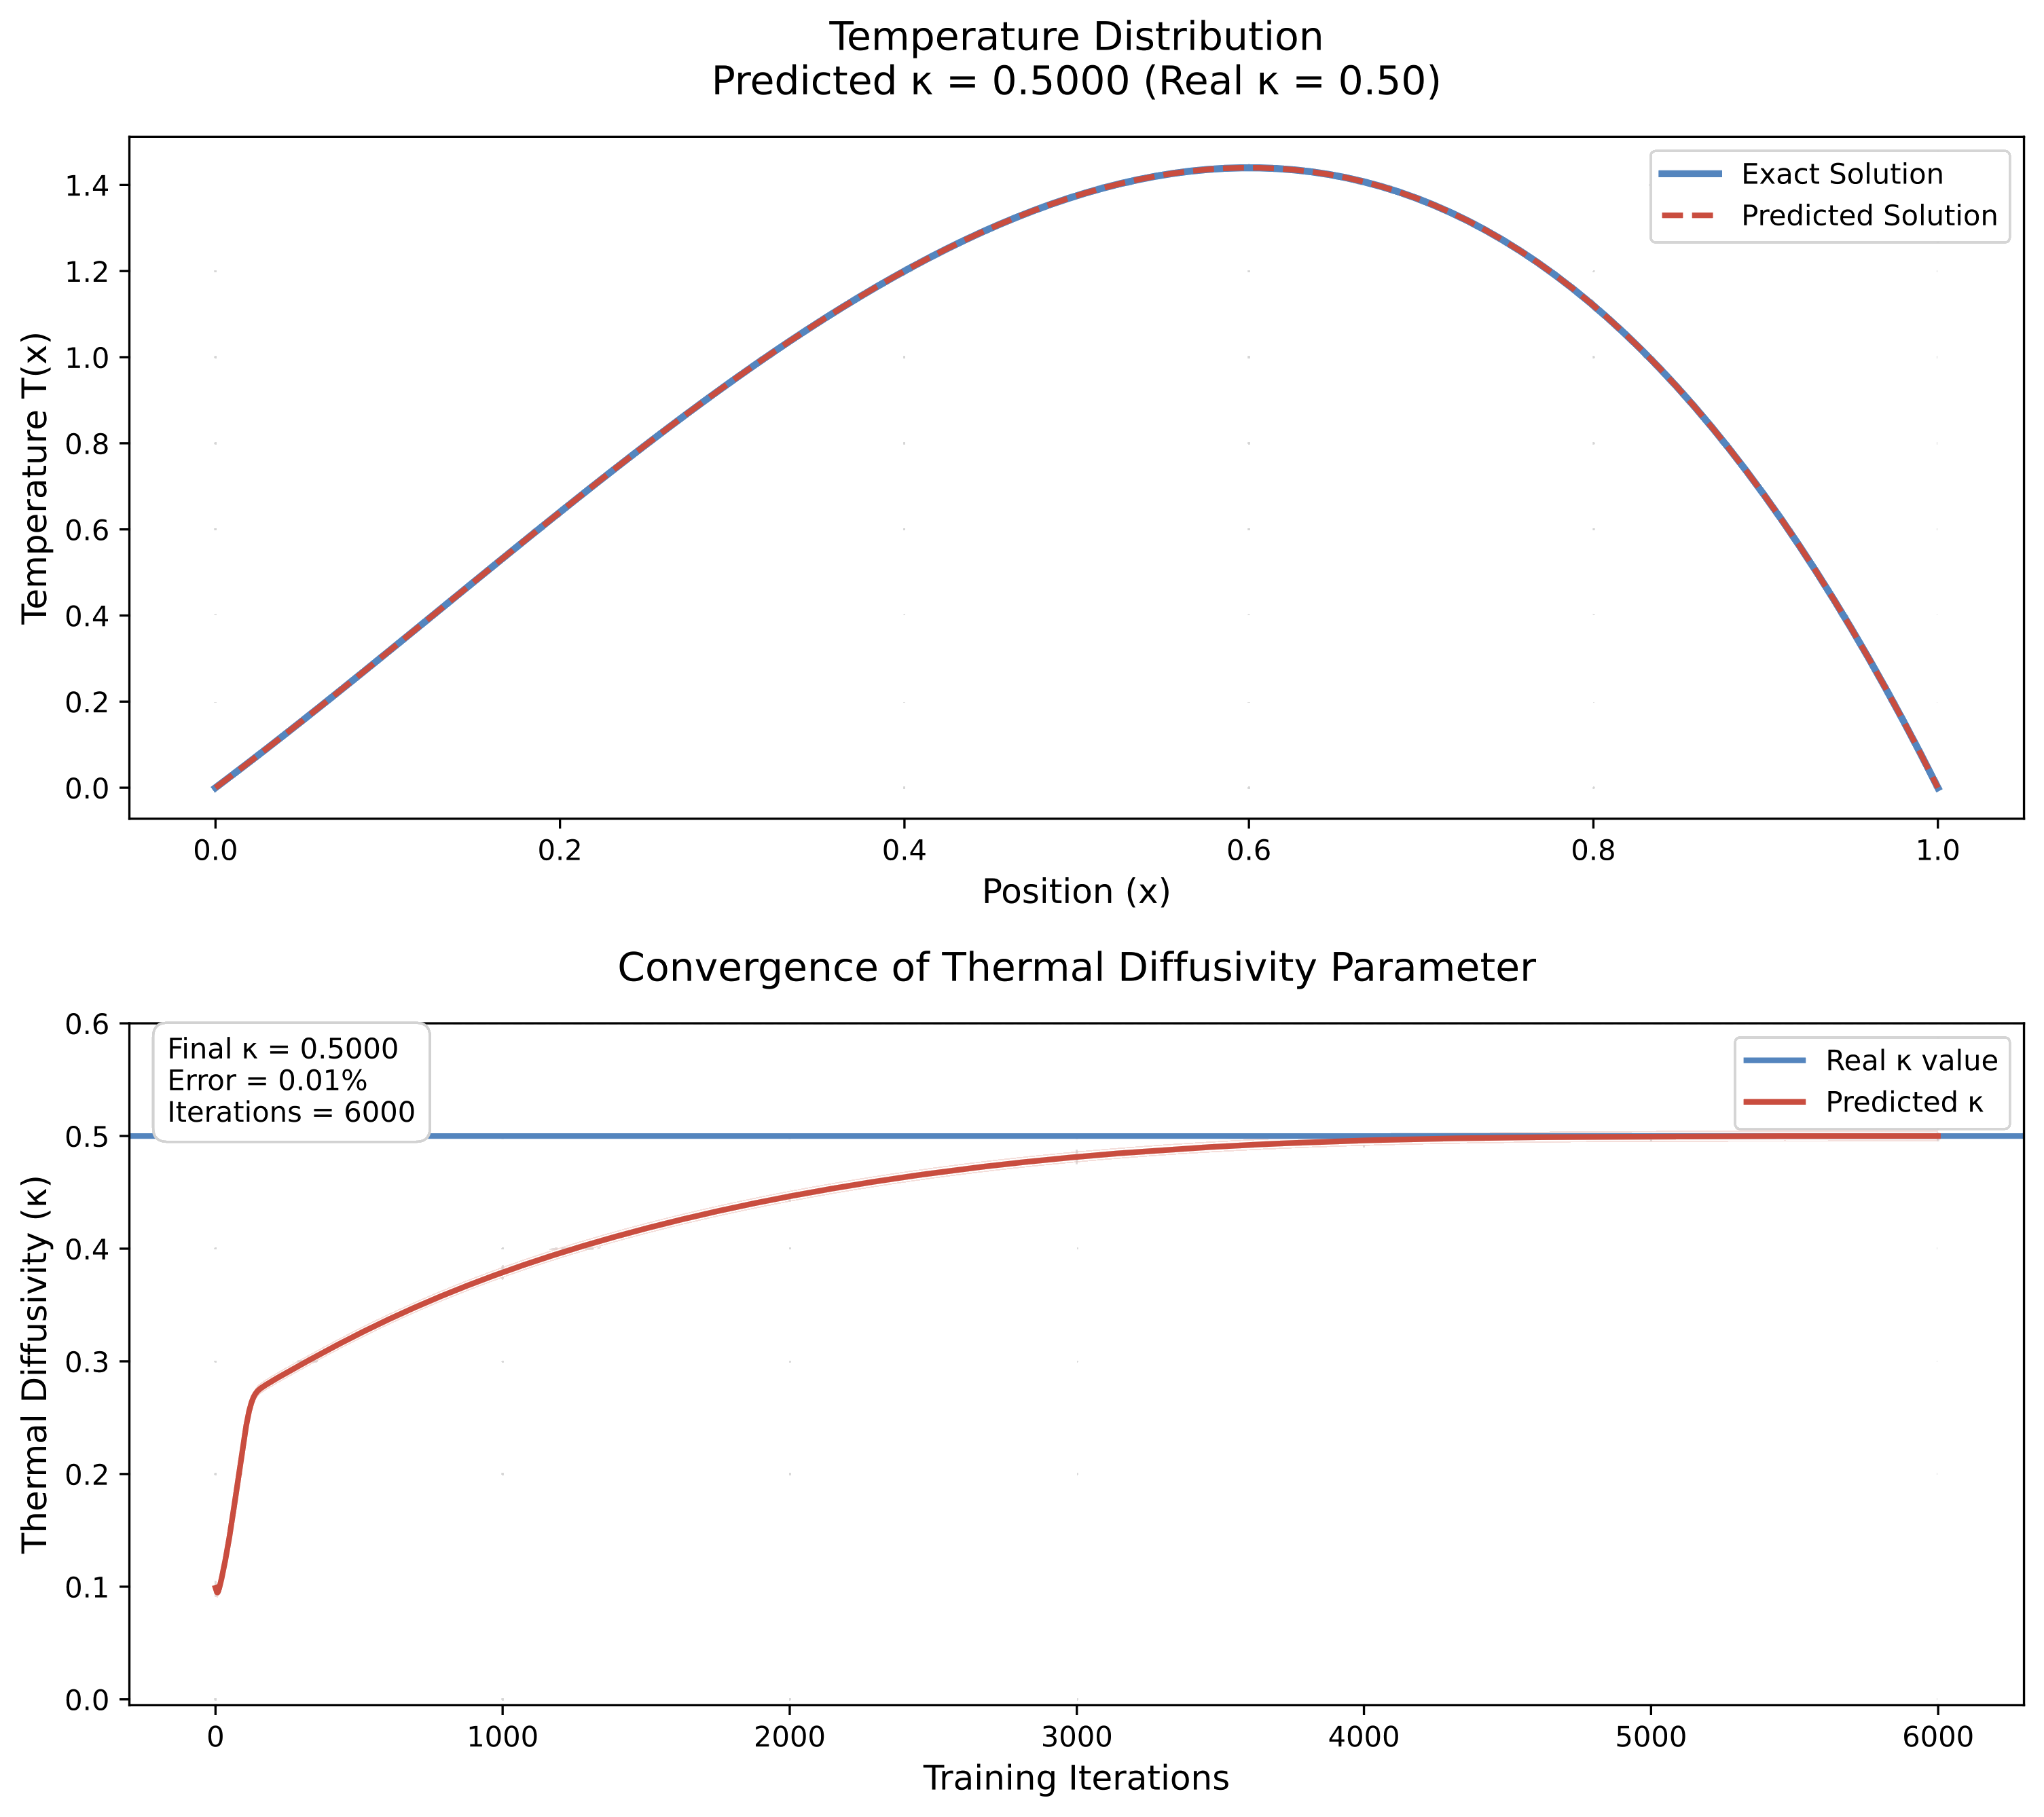
\includegraphics[width=0.75\textwidth]{figs/inverse-heat-diffusivity.png}
	\end{figure}
	
\end{frame}

%------------------------------------------------
\begin{frame}
\frametitle{The PINN Approach to Inverse Problems}

\textbf{The Key Insight:} Treat the unknown physical parameters as additional trainable variables in the network.

\textbf{Problem:} 1D steady-state heat conduction.
\begin{equation*}
-k \frac{d^2T}{dx^2} = f(x)
\end{equation*}
Here, the thermal diffusivity $k$ is \textbf{unknown}.

\textbf{PINN Framework:}
\begin{itemize}
    \item The neural network learns the temperature field: $\hat{T}_\theta(x)$.
    \item A new trainable parameter is introduced: $\hat{k}$.
    \item The optimizer updates both the network weights $\theta$ and the parameter $\hat{k}$ simultaneously.
\end{itemize}

\textbf{Loss Function:} $\mathcal{L}(\theta, \hat{k}) = \mathcal{L}_{\text{data}} + \mathcal{L}_{\text{PDE}} + \mathcal{L}_{\text{BC}}$
where the physics loss now includes the trainable parameter $\hat{k}$:
\begin{equation*}
\mathcal{L}_{\text{PDE}} = \frac{1}{N_f}\sum \left|-\hat{k}\frac{d^2\hat{T}_\theta}{dx^2}(x_j) - f(x_j)\right|^2
\end{equation*}

\end{frame}

%------------------------------------------------
\begin{frame}
\frametitle{Implementation: Parameter Estimation}

\begin{figure}[ht]
	\centering
	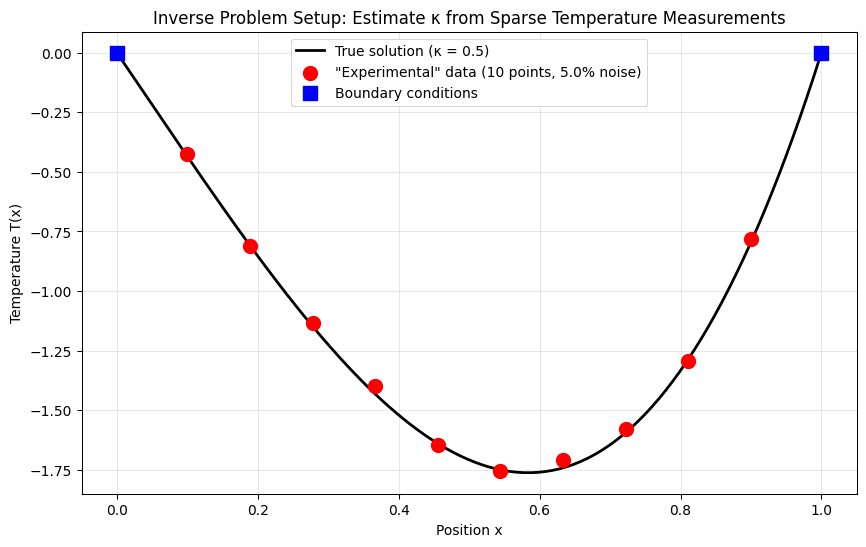
\includegraphics[width=0.9\textwidth]{figs/inverse-problem-setup.png}
	\caption*{"Experimental Setup" plot, showing the true solution and sparse, noisy data points.}
\end{figure}

\textbf{Challenge:} Can the PINN recover the true value of $k$ from only 10 noisy measurements?

\end{frame}

%------------------------------------------------
\begin{frame}
\frametitle{Results: Parameter Recovery}

\begin{minipage}[t]{0.48\textwidth}
\begin{figure}[ht]
	\centering
	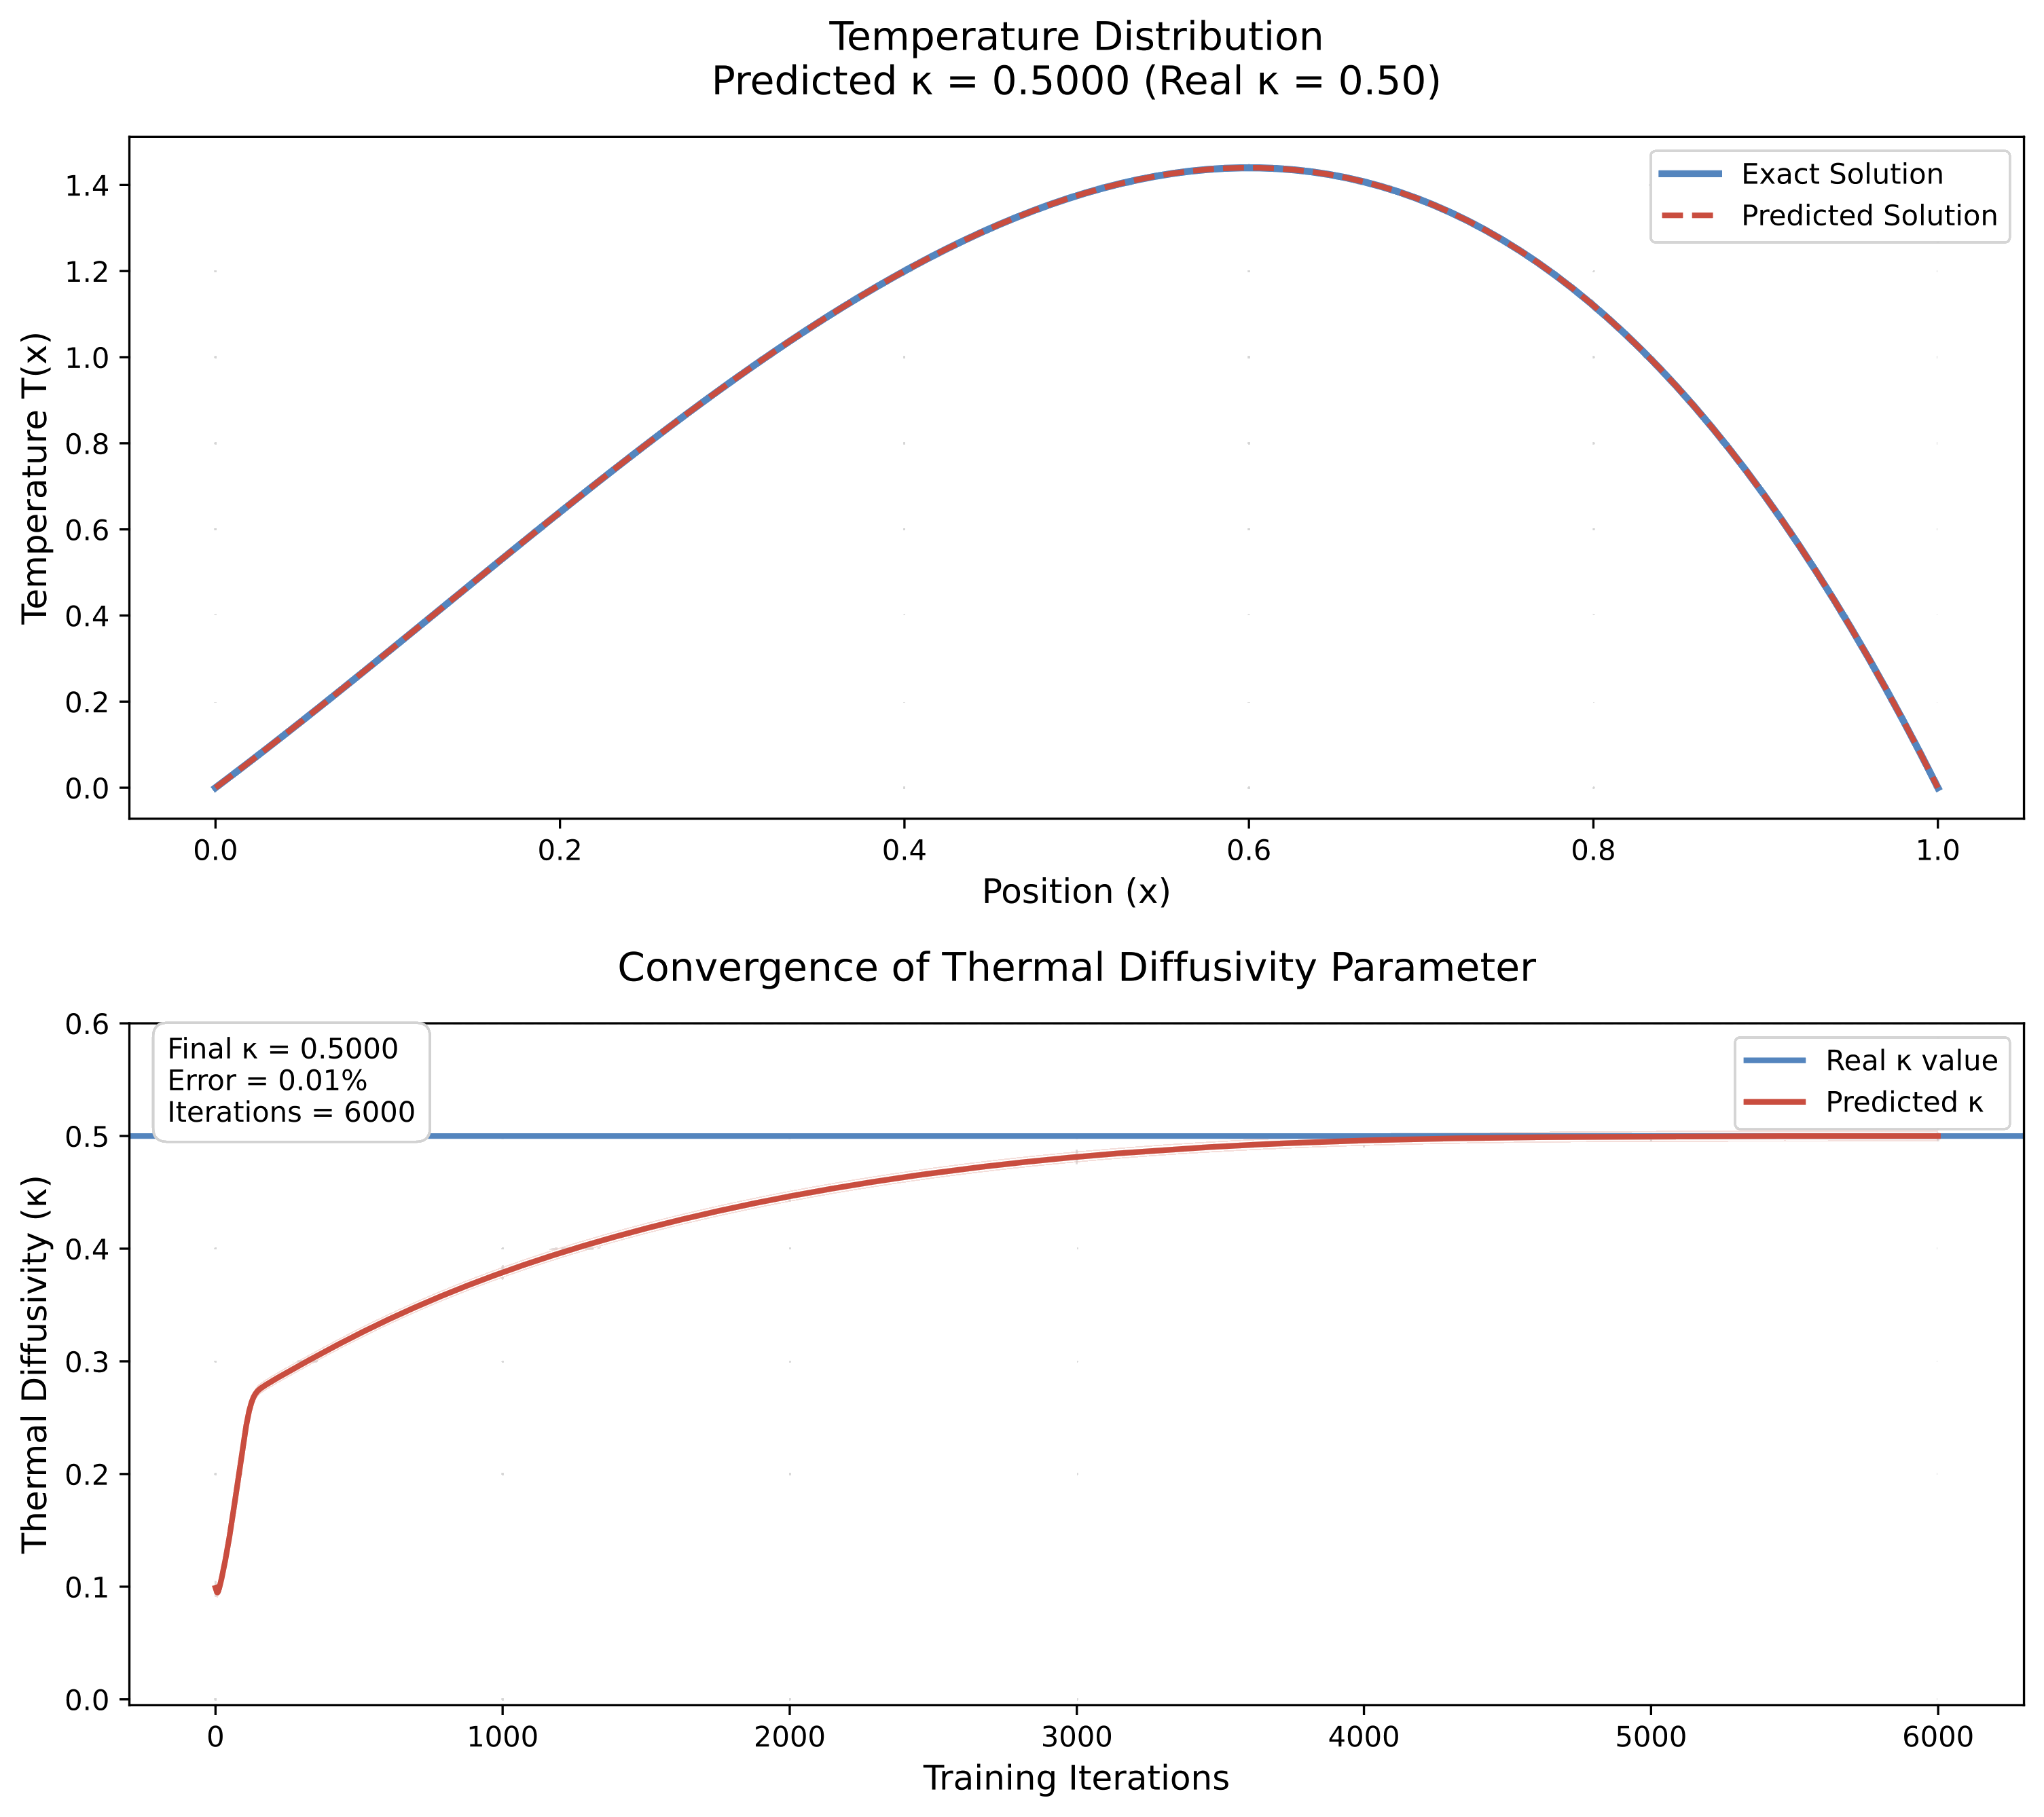
\includegraphics[width=\linewidth]{figs/inverse-heat-diffusivity.png}
	\caption*{Parameter convergence and temperature field reconstruction.}
\end{figure}
\end{minipage}
\hfill
\begin{minipage}[t]{0.48\textwidth}
\begin{itemize}
    \item The estimated parameter $\hat{k}$ converges to the true value.
    \item The PINN simultaneously reconstructs the full, continuous temperature field accurately.
    \item This is achieved from very sparse and noisy data, showcasing the regularizing effect of the physics loss.
\end{itemize}
\end{minipage}

\end{frame}

%------------------------------------------------
\begin{frame}
\frametitle{Summary: Why PINNs are Powerful}

\textbf{1. Regularization Effect:}
\begin{itemize}
    \item Physics constraints prevent overfitting and guide the solution in data-sparse regions.
\end{itemize}

\textbf{2. Data Efficiency:}
\begin{itemize}
    \item Physics provides a strong inductive bias, allowing PINNs to learn from very few measurements.
\end{itemize}

\textbf{3. Accurate Derivatives:}
\begin{itemize}
    \item Automatic differentiation provides exact derivatives, which are learned correctly as a consequence of enforcing the physics.
\end{itemize}

\textbf{4. Versatility:}
\begin{itemize}
    \item The same framework can solve forward problems, inverse problems, and handle various boundary conditions.
\end{itemize}

\begin{center}
\textbf{PINNs = Universal Function Approx. + Physics Constraints + Auto. Diff.}
\end{center}

\end{frame}

%------------------------------------------------
\begin{frame}
\frametitle{Questions?}

\centering
\Large Thank you!

\vspace{2cm}

\textbf{Contact:} \\
Krishna Kumar \\
\textit{krishnak@utexas.edu} \\
University of Texas at Austin

\end{frame}

\end{document}